\section{Polygonal Meshes}
\label{sec:polygonal}

In this section, we introduce polygonal meshes, describe a data structure to efficiently
work with them, and define the Euler characteristic.

\subsection{What is a surface?}

 Many surfaces are made up of many vertices, edges, and
triangles (or other polygons). An example of a triangular mesh is shown in \figref{cat}.


 \begin{figure}[htb]
         \centering
        \begin{subfigure}[b]{0.3\textwidth}
         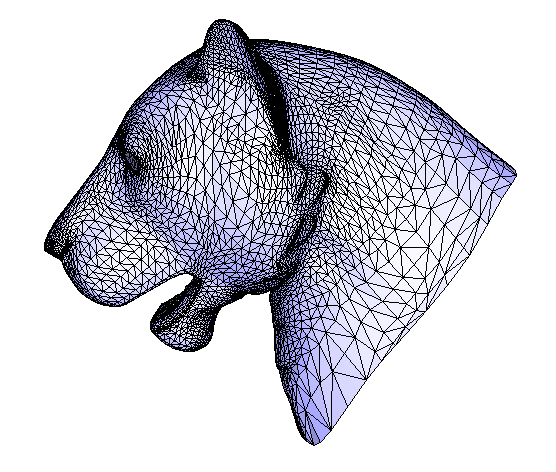
\includegraphics[width=\textwidth]{polygonal-mesh/profile}
         \caption{}
 	 \label{fig:profile}
       \end{subfigure}
         \hspace{.6cm}
         \begin{subfigure}[b]{0.19\textwidth}
         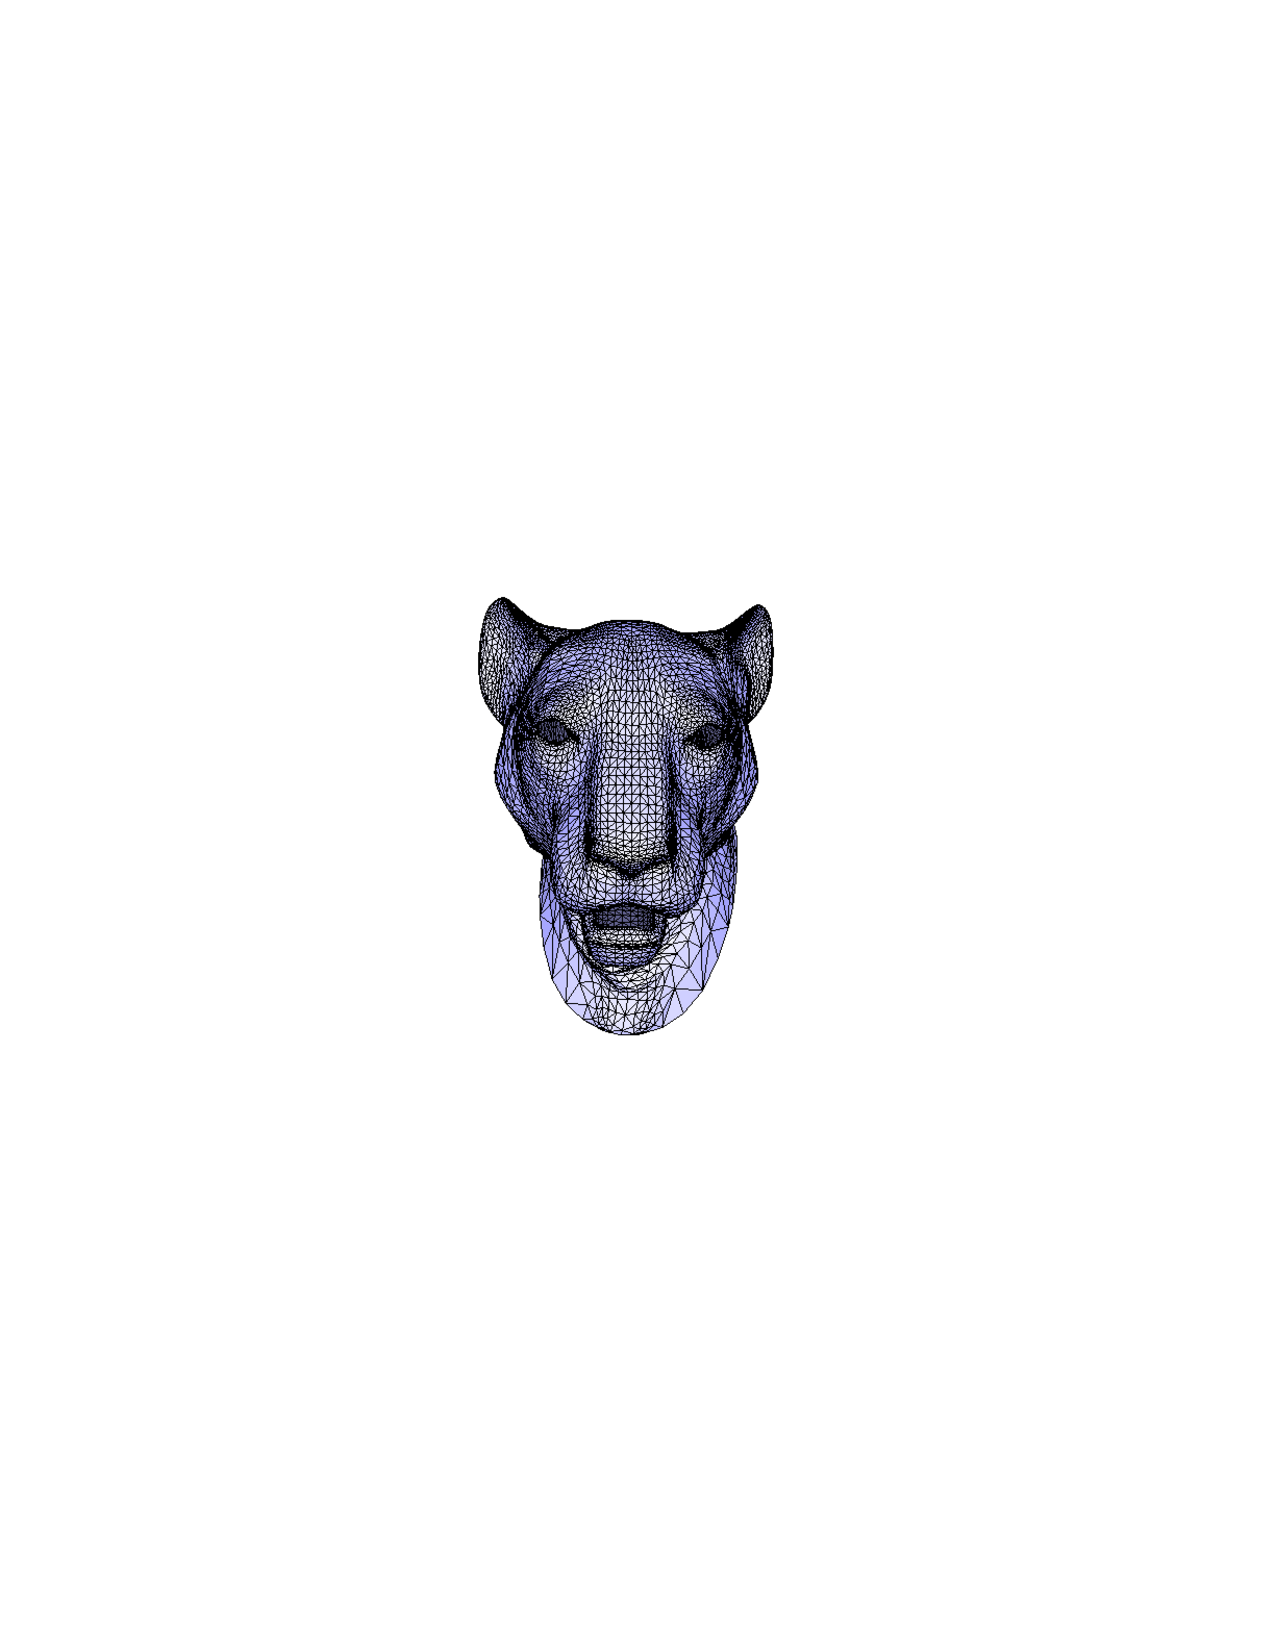
\includegraphics[width=\textwidth]{polygonal-mesh/head-on}
         \caption{}
          \label{fig:head-on}
         \end{subfigure}
             \hspace{.6cm}
         \begin{subfigure}[b]{0.24\textwidth}
         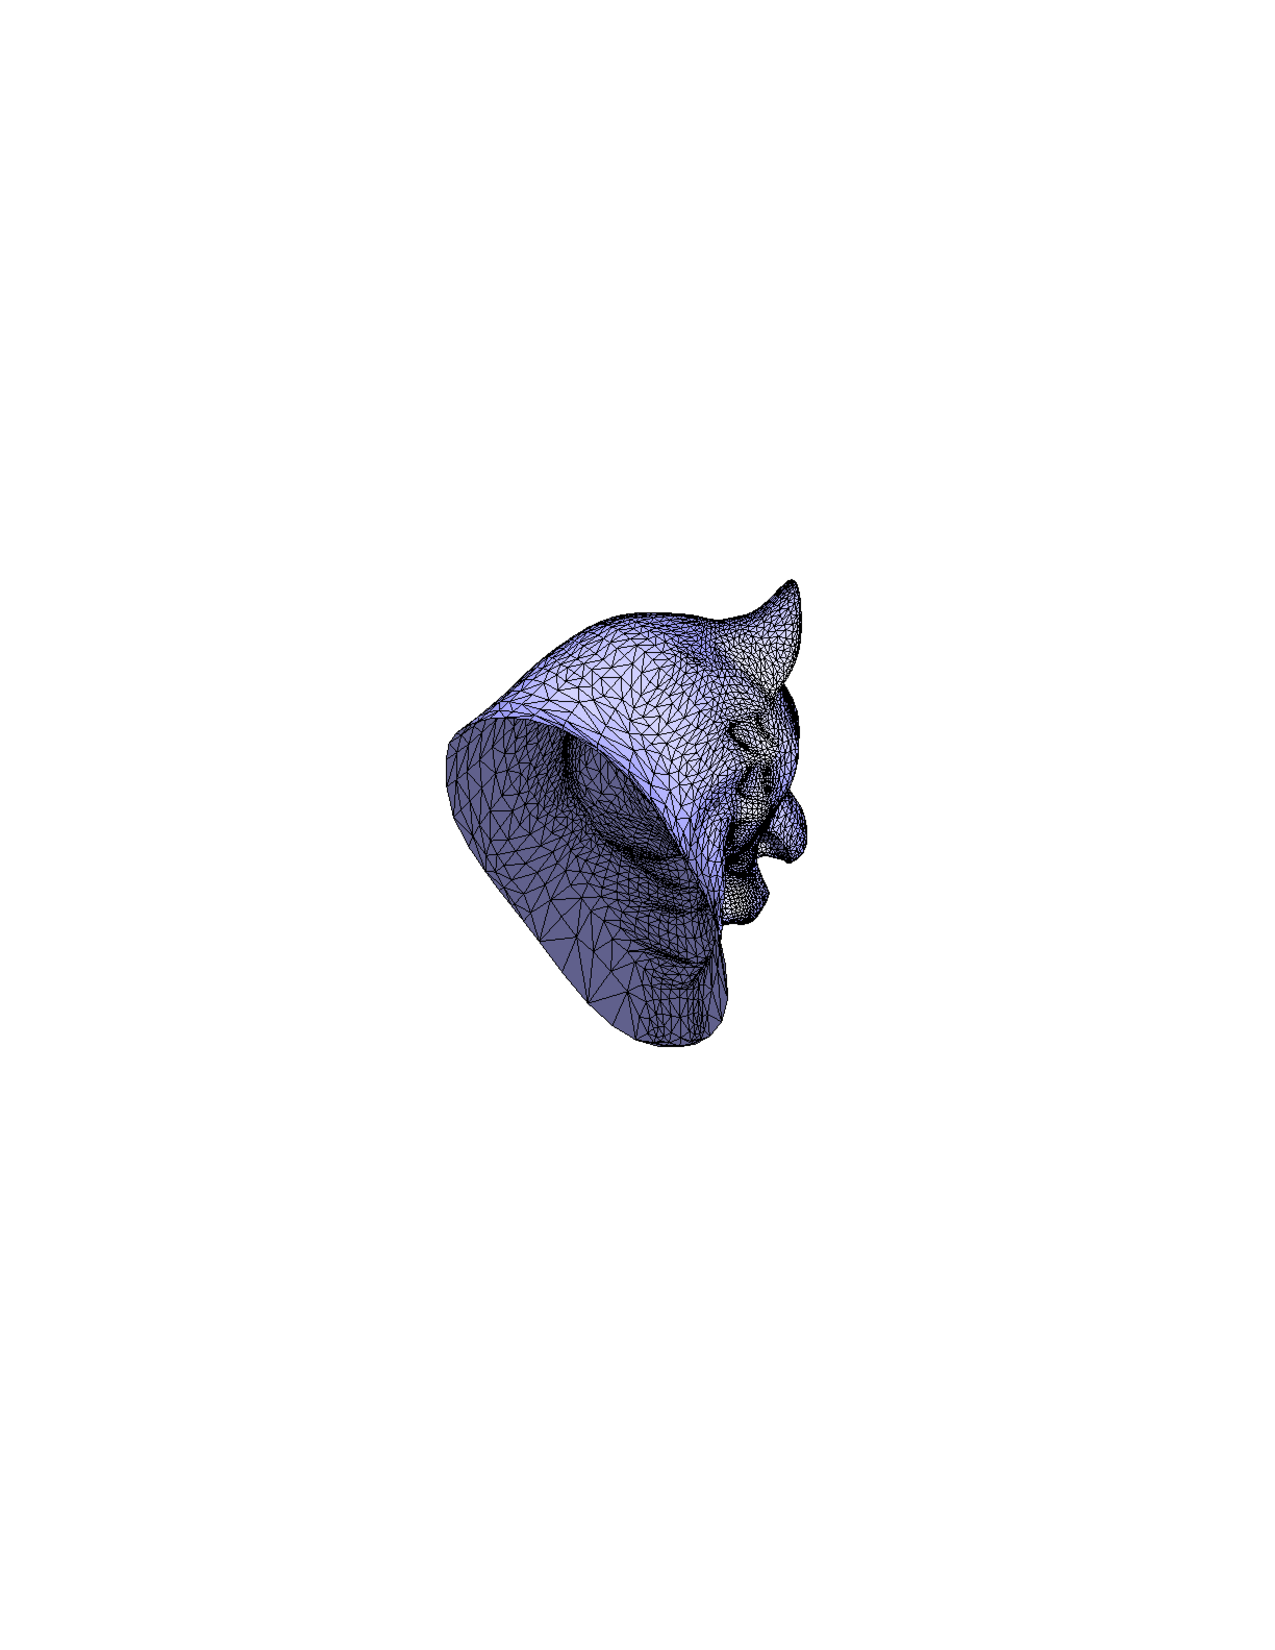
\includegraphics[width=\textwidth]{polygonal-mesh/back}
         \caption{}
          \label{fig:back}
         \end{subfigure}
		\caption{(\subref{fig:profile}) A profile view of a mesh.
 		(\subref{fig:head-on})  A head on view of the same mesh and the view from the back (\subref{fig:back}).
 		\label{fig:cat}}
 \end{figure}

One way to store a mesh in a computer is as a OFF file.
The first optional line of an OFF file identifies the file as an OFF file.
The second line lists the number of vertices, faces, and edges.
A list of vertices in $(x,y,z)$ coordinates is then given followed
by a list of faces indicated by the index of the vertices contained in the face.
For the mesh in \figref{cat}, the OFF file looks is shown in 
\tabref{off}.

\begin{table}[h!]
\caption{The OFF data for the mesh in \figref{cat}.}
\centering
\begin{tabular}{|p{2cm} p{2cm} p{2cm} p{2cm}|} 
 \hline
OFF &  & &  \\ 
7529 & 14859 & 0 &  \\ 
-0.29196 & -0.0867173 & -0.355149  &  \\
 -0.123586   & -0.0127199 & -0.385597 &  \\
-0.138255   & -0.0985078 & -0.384018 &  \\
  & &\vdots &  \\  
 3&  97 &1893& 1895\\
 3& 71 & 1894 & 1893 \\
 3 & 16 & 1895 & 1894\\
   & &\vdots &  \\  
 \hline
\end{tabular}

\label{tab:off}
\end{table}


\noindent \textbf{Exercises}


\begin{enumerate}
	\item 
	
\end{enumerate}

\pagebreak